\documentclass[tikz,border=5mm]{standalone}
\usepackage{tikz}
\usetikzlibrary{arrows.meta, positioning, shapes.geometric, calc, patterns}

% --- COLOR DEFINITIONS ---
\definecolor{Garnet}{HTML}{73000A}
\definecolor{CBlue}{HTML}{466A9F}
\definecolor{CDark}{HTML}{1F414D}
\definecolor{CGold}{HTML}{A49137}
\definecolor{CGrayLight}{HTML}{E5E5E5}
\definecolor{CGrayDark}{HTML}{555555}
\definecolor{CWhite}{HTML}{FFFFFF}

\begin{document}

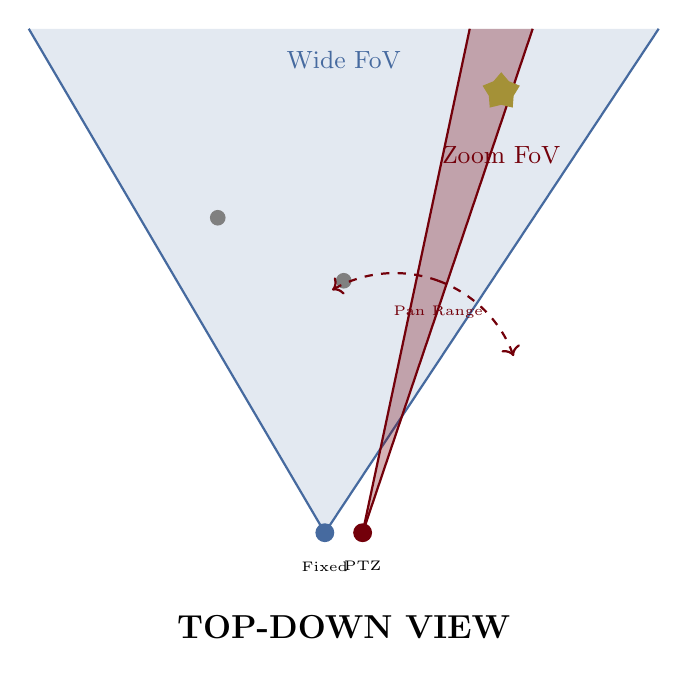
\begin{tikzpicture}[scale=0.8]
    % Title
    \node[font=\bfseries\large] at (0, -1.5) {TOP-DOWN VIEW};
    
    % Cameras (simple dots, side by side)
    \fill[CBlue] (-0.3, 0) circle (0.15);
    \fill[Garnet] (0.3, 0) circle (0.15);
    \node[below, font=\tiny] at (-0.3, -0.3) {Fixed};
    \node[below, font=\tiny] at (0.3, -0.3) {PTZ};
    
    % Wide FOV (Blue) - Large triangle pointing up
    \fill[CBlue, opacity=0.15] (-0.3, 0) -- (-5, 8) -- (5, 8) -- cycle;
    \draw[CBlue, thick] (-0.3, 0) -- (-5, 8);
    \draw[CBlue, thick] (-0.3, 0) -- (5, 8);
    \node[CBlue, font=\small] at (0, 7.5) {Wide FoV};
    
    % Zoom FOV (Red) - Narrow triangle INSIDE the blue one
    % Currently pointing slightly to the right
    \fill[Garnet, opacity=0.3] (0.3, 0) -- (2, 8) -- (3, 8) -- cycle;
    \draw[Garnet, thick] (0.3, 0) -- (2, 8);
    \draw[Garnet, thick] (0.3, 0) -- (3, 8);
    \node[Garnet, font=\small] at (2.5, 6) {Zoom FoV};
    
    % Target inside zoom beam
    \node[star, star points=5, fill=CGold, minimum size=0.4cm] at (2.5, 7) {};
    
    % Other objects in wide FOV but outside zoom
    \node[circle, fill=gray, inner sep=2pt] at (-2, 5) {};
    \node[circle, fill=gray, inner sep=2pt] at (0, 4) {};
    
    % Pan arrows showing zoom can move
    \draw[->, Garnet, dashed, thick] (1.5, 4) arc (70:20:2);
    \draw[->, Garnet, dashed, thick] (1.5, 4) arc (70:120:2);
    \node[Garnet, font=\tiny] at (1.5, 3.5) {Pan Range};
    
\end{tikzpicture}

\end{document}
